\documentclass[10pt]{article}

\usepackage{spheric}
%%%TITLE
\title{SPH for the interaction between tsunami wave and upright cylindrical groups}
\date{}

%%AFFILIATIONS
\author[$\relax$]{Jing-jun Li$^\dagger$}
\author[$\relax$]{Lei Tian}
\author[$\relax$]{Yongsen Yang}
\author[$\relax$]{Liu-Chao Qiu}
\author[$\relax$]{Yu Han}
\affil[$\relax$]{China Agricultural University, China}
\affil[$\relax$]{\email{\dagger}{LiJingjunedu@163.com}}


%%DOCUMENT
\begin{document}

\maketitle

%\SelectedTopics{}

%%PLEASE PUT YOUR ABSTRACT HERE
\begin{abstract}
The Smoothed Particle Hydrodynamics (SPH) method has proven to have great potential in dealing with the wave-structure interactions since it can deal with the large amplitude and easily captures the free surface. Based on the sph method, this paper verifies the accuracy of a piston-type wave maker and its generated wave force by simulating two experiments, which gives very satisfactory results. The focus of the study is the wave interaction with upright cylindrical groups. The weakening effect of the upright cylindrical group on the waves is found though the simulation by SPH. And with the increase in the number of cylindrical layers, the ability to weaken the waves is enhanced.

\begin{figure}[!htb]
\centering
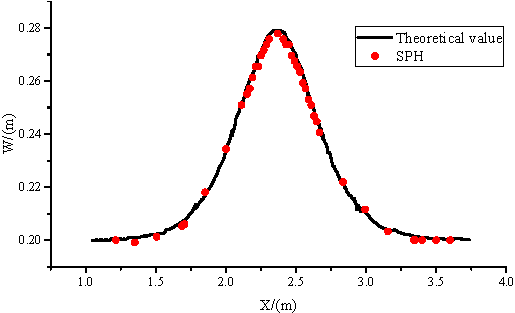
\includegraphics[width=0.5\textwidth]{46-1.pdf}
\caption{Validation of piston-type wave maker condition in SPH}\label{fig:46-1}
\end{figure}

The comparison between the theoretical and simulated values of the wave height verifies the piston-type wave maker by sph is accurate.

\begin{figure}[!htb]
\centering
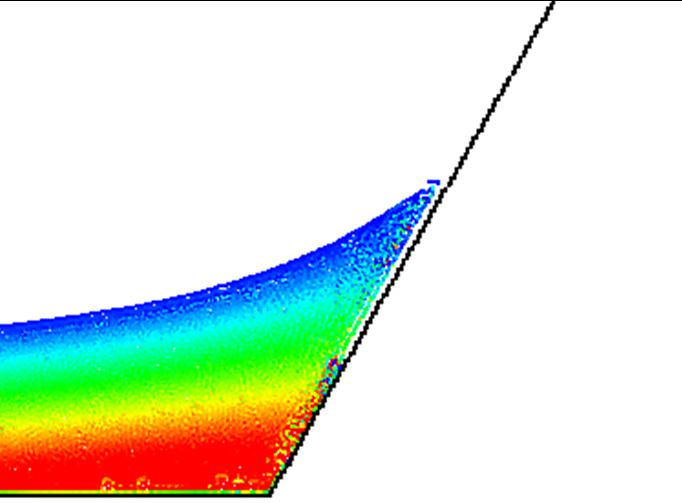
\includegraphics[width=0.46\textwidth]{46-21.png}~~~
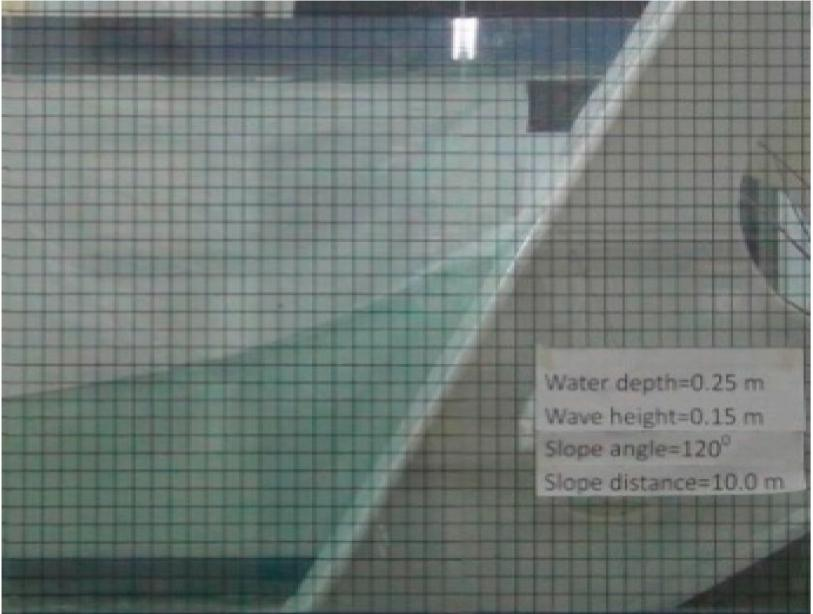
\includegraphics[width=0.46\textwidth]{46-22.png}
\caption{The interaction between waves and slopes: Comparison of SPH (left) to experimental value (right)}\label{fig:46-2}
\end{figure}

\end{abstract}


%%THE END OF ABSTRACT

\addbib

\end{document}
